\chapter{Kademlia}
\textbf{Kademlia} is a protocol used by some of the largest public DHTs
\note{
   \ns
\begin{itemize}
   \item BitTorrent Mainline DHT
   \item Ethereum P2P network
   \item IPFS
\end{itemize}
}
It has three key charateristics which are not offered by other DHTs
\begin{enumerate}
   \item routing information spreads automatically as a side-effect of lookups
   \item flexibility to send multiple requests in parallel to speed up lookups by
   avoiding timeout delays (parallel routing)
   \item iterative routing
   \note{At each routing step of the query, the queried node sends a report to the starting querying node, even if it could not answer the query.}
\end{enumerate}

\section{Structure}
\begin{paracol}{2}
   \colfill
   Kademlia exploits the leaves of a \textbf{Trie}\footnote{k-ary search tree and prefix tree} to define the logical identifier space;

   Note that not all leaves correspond to nodes (peers)
   \colfill
   \switchcolumn

   \begin{figure}[htbp]
      \centering
      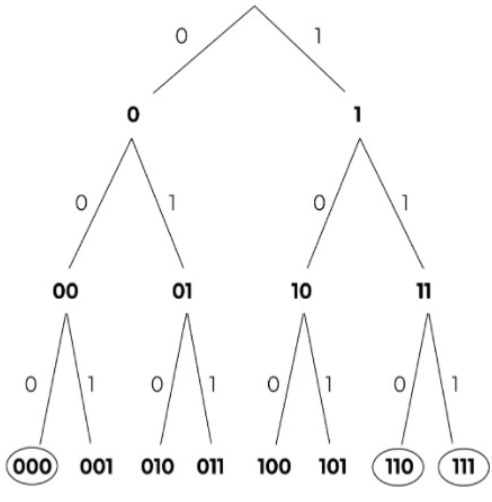
\includegraphics{images/kademlia_trie.png}
      \caption{Trie}
      \label{fig:kademlia_trie}
   \end{figure}
\end{paracol}

\subsection{Assigning keys to leaves}
The rule to partition the keys (content) among the nodes must respect the rules of \textit{consistent hashing}.

\begin{paracol}{2}
   \begin{definition}[Partitioning rule]
      A key is assigned to the node with the
      \textit{``\ul{lowest} common ancestor''}:\\
      Find the longest prefix between the
      key and the node identifier, and then assign the key to such node.
   \end{definition}
   \switchcolumn
   \begin{figure}[htbp]
      \centering
      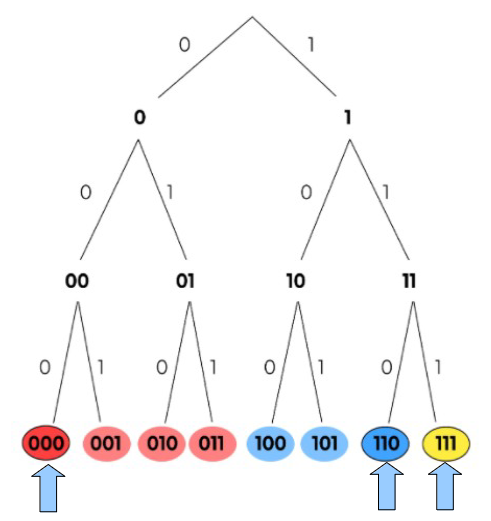
\includegraphics[width=0.45\columnwidth]{images/kademlia_leaves01.png}
      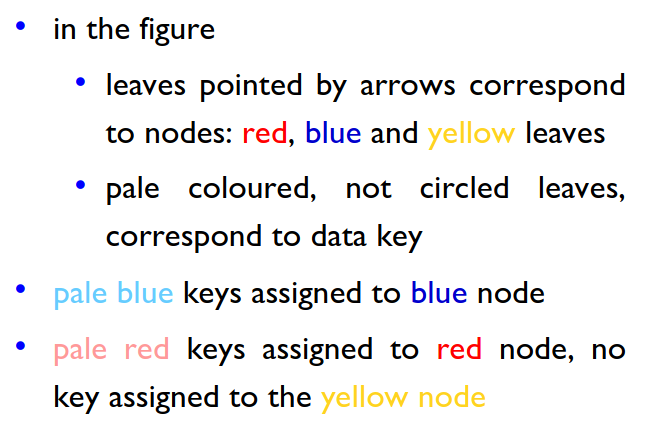
\includegraphics[width=0.45\columnwidth]{images/kademlia_leaves02.png}
      \label{fig:kademlia_leaves}
   \end{figure}
\end{paracol}

\section{XOR Metric}

TODO

\section{Routing Table}
In order to look for data, Kademlia's key idea is to \ul{store a logarithmic number of node IDs and their corresponding IP} addresses and some contact taken from the identifier trie.

